\documentclass{elektr}
\usepackage{hyperref}
\hypersetup{
colorlinks=true,
urlcolor=blue,
citecolor=blue}
\usepackage[all]{xy,xypic}
\usepackage{amsfonts,amssymb,amsmath,amsgen,amsopn,amsbsy,theorem,graphicx,epsfig}
\usepackage{eufrak,amscd,bezier,latexsym,mathrsfs,eurosym,enumerate}
\usepackage[utf8]{inputenc}
\usepackage[english]{babel}
\usepackage{cleveref,multirow}
\usepackage[dvipsnames]{xcolor}
\usepackage[pagewise]{lineno}
\linenumbers

\yil{}
\vol{}
\fpage{}
\lpage{}
\doi{}

\title{Manuscript template: full title must be in sentence case}

\author[]{
	\rec{.202}
	\acc{.202}
	\finv{..202}
}

\def\E{\ifmmode{\mathbb E}\else{$\mathbb E$}\fi} %natural numbers
\def\N{\ifmmode{\mathbb N}\else{$\mathbb N$}\fi} %natural numbers
\def\R{\ifmmode{\mathbb R}\else{$\mathbb R$}\fi} %real numbers
\def\Q{\ifmmode{\mathbb Q}\else{$\mathbb Q$}\fi} %rational numbers
\def\C{\ifmmode{\mathbb C}\else{$\mathbb C$}\fi} %complex numbers
\def\H{\ifmmode{\mathbb H}\else{$\mathbb H$}\fi} %complex numbers
\def\Z{\ifmmode{\mathbb Z}\else{$\mathbb Z$}\fi} %integers
\def\P{\ifmmode{\mathbb P}\else{$\mathbb P$}\fi} %real numbers
\def\T{\ifmmode{\mathbb T}\else{$\mathbb T$}\fi} %real numbers
\def\SS{\ifmmode{\mathbb S}\else{$\mathbb S$}\fi} %real numbers
\def\DD{\ifmmode{\mathbb D}\else{$\mathbb D$}\fi} %real numbers

\renewcommand{\a}{\alpha}
\renewcommand{\b}{\beta}
\renewcommand{\d}{\delta}
\newcommand{\D}{\Delta}
\newcommand{\e}{\epsilon}
\newcommand{\var}{\varepsilon}
\newcommand{\g}{\gamma}
\newcommand{\la}{\lambda}
\newcommand{\La}{\Lambda}
\newcommand{\lan}{\langle}
\newcommand{\ran}{\rangle}
\newcommand{\n}{\nabla}
\newcommand{\va}{\varphi}
\newcommand{\s}{\sigma}
\newcommand{\Sig}{\Sigma}
\renewcommand{\t}{\tau}
\renewcommand{\th}{\theta}
\newcommand{\Om}{\Omega}
\newcommand{\om}{\omega}
\newcommand{\pa}{\partial}
\newcommand{\up}{\upsilon}
\newcommand{\vp}{\varphi}
\newcommand{\z}{\zeta}





\newcommand{\bse}{\begin{subequations}}
\newcommand{\ese}{\end{subequations}}
\newcommand{\ben}{\begin{enumerate}}
\newcommand{\een}{\end{enumerate}}
\newcommand{\bens}{\begin{enumerate*}}
\newcommand{\eens}{\end{enumerate*}}
\newcommand{\be}{\begin{equation}}
\newcommand{\ee}{\end{equation}}
\newcommand{\bea}{\begin{eqnarray}}
\newcommand{\eea}{\end{eqnarray}}
\newcommand{\baa}{\begin{eqnarray*}}
\newcommand{\eaa}{\end{eqnarray*}}
\newcommand{\bc}{\begin{center}}
\newcommand{\ec}{\end{center}}
\newcommand{\ol}{\overline}
\newcommand{\ul}{\underline}
\newcommand{\ov}{\overbrace}
\newcommand{\uv}{\underbrace}
\newcommand{\Ra}{\Rightarrow}
\newcommand{\ra}{\rightarrow}
\newcommand{\ds}{\displaystyle}
\newcommand{\vs}{\vspace}


\newcommand{\IR}{\mbox{I \hspace{-0.2cm}R}}
\newcommand{\IN}{\mbox{I \hspace{-0.2cm}N}}



%% \theoremstyle{plain} %% This is the default

\newtheorem{theorem}{Theorem}%[section]

\theoremstyle{corollary}
\newtheorem{corollary}{Corollary}

\theoremstyle{lemma}
\newtheorem{lemma}{Lemma}

\theoremstyle{proposition}
\newtheorem{proposition}{Proposition}

\theoremstyle{axiom}
\newtheorem{axiom}{Axiom}

\theoremstyle{conjecture}
\newtheorem{conjecture}{Conjecture}

\theoremstyle{example}
\newtheorem{example}{Example}

\theoremstyle{definition}
\newtheorem{definition}{Definition}%[section]

\theoremstyle{remark}
\newtheorem{remark}{Remark}%[section]
\newtheorem{notation}{Notation}


\newtheorem{question}{Question}%[section]
\newtheorem{construction}{Construction}

\newtheorem{athm}{Theorem}
\renewcommand{\theathm}{\Alph{athm}}





\setcounter{page}{1}
\begin{document}

\maketitle


\begin{abstract}This document is a template for use by authors sending manuscripts to the Turkish Journal of Electrical Engineering {\&} Computer Sciences. It also contains important information on the paper style. The title of the manuscript must be written in lower case except for the first word and proper nouns. Author names must be given in full, with surnames (family names) all in capitals. Author addresses must be given in English in the following order: Department, Faculty, University, City, Country, with numbers in superscript after each author name to indicate his/her address. Footnotes must not be used for addresses. The corresponding author's email address must be clearly given, marked with an asterisk. The abstract must not be longer than 300 words and must clearly state the study's purpose and results. The manuscript's title and abstract must not contain mathematical formulae. The abstract must not contain any reference citations. The key words must be separated by commas and should not include acronyms.

\keywords{Electronics, instructions for authors, manuscript template}
\end{abstract}

\section{Introduction}
\label{Int}

Authors should use this template very carefully when preparing a manuscript for submission to the Turkish Journal of Electrical Engineering {\&} Computer Sciences. The manuscript should be written in \LaTeX. \textbf{Starting in January 2018, other formats are not accepted.} The text in this template can be replaced by typing or copy/pasting to form the final form of the manuscript. The style of this document should never be changed. Please make sure that, in addition to this template, you carefully read and follow the ``Instructions for Authors'' in the journal web site. Submissions that do not strictly follow this template and/or all instructions for authors are returned back to authors without review.

\subsection{Sections and subsections}

Articles should be divided into sections and subsections. Principal sections should be numbered consecutively (e.g., as 1. Introduction, 2. Materials and methods, etc.), while subsections should be numbered as 1.1., 1.2., etc. Do not use numbers for the Acknowledgments and References sections. \textbf{The total number of pages for the abstract, all sections (e.g., Introduction, Materials and methods, Results, Discussion, etc.), references, tables, and figures should not exceed {\Large 15}. For this journal, one of the most common return reason during initial submissions is exceeding the number of pages. The number of pages is strictly limited; because, this journal is free of charge (for both authors and readers).} 

The Introduction should argue the case for the study, outlining only essential background, and should not include details of findings or conclusions. It should not be only a review of the subject area, but it should also contain a clear statement of the question being addressed. In the Materials and methods section, please provide concise but complete information on materials and analytical/statistical procedures used. This part should be as clear as possible to enable other scientists to repeat the research presented. For example, brand names and company locations should be supplied for all mentioned equipment, instruments, chemicals, etc. Results of the study should be given in the Results section. In the Discussion section, where findings are discussed, statements from the Introduction and Results sections should not be repeated unnecessarily. It is advised that the final paragraph of the Discussion section highlights the main conclusions of the study. The Results and Discussion sections may be combined. Where necessary, you can refer to sections like Section~\ref{Int}.

\begin{figure}[h!]
\begin{center}
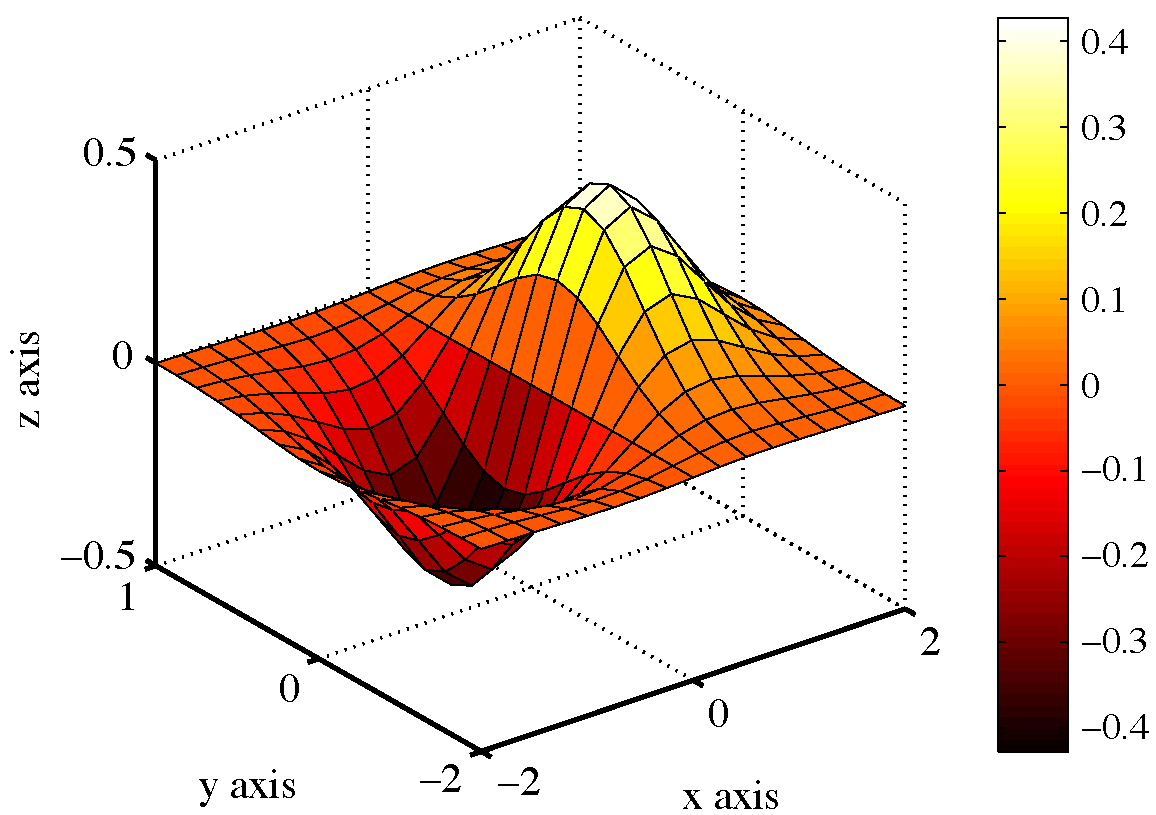
\includegraphics[width=9.0cm]{figure_example}
\caption{A sample figure.}
\label{fig1}
\end{center}\vs{-4mm}
\end{figure}

Manuscripts must be written in English. Contributors who are not native English speakers are strongly advised to ensure that a colleague fluent in the English language or a professional language editor has reviewed their manuscript. Concise English without jargon should be used. Repetitive use of long sentences and passive voices should be avoided. It is strongly recommended that the text be run through computer spelling and grammar programs. Either British or American spelling is acceptable but it must be consistent throughout. Manuscripts written in poor English will not be submitted to referees for evaluation and will be returned back to authors.  

\textbf{We emphasize that the style of this document, including line spacing, margins, fonts, and page numbers, should never be changed.}  

\subsection{Symbols, units, and abbreviations}

In general, this journal follows the conventions of \textit{Scientific Style and Format, The CSE Manual for Authors, Editors, and Publishers, Council of Science Editors, Reston, VA, USA}. All symbols, such as $\times, \mu, \eta$, and $\nu$, should be written by using corresponding \LaTeX definitions. For example, the degree symbol should be used as $^{\circ}$ and it should not be written by using superscripted letter o or number 0. Similarly, the multiplication symbol must be used as $\times$, not the letter x. Spaces must be inserted between numbers and units (e.g., $3$~kg, $2$~m, $10$~V) and between numbers and mathematical symbols (e.g., $+$, $-$, $\times$, $=$, $<$, $>$), but not between numbers and percent symbols (e.g., 45{\%} is the correct version). Please use SI units. All abbreviations and acronyms should be defined at the first mention. Latin terms such as et al., in vitro, and in situ, should not be italicized. 

\begin{table}[h!]
\caption{A sample table including some styles.}
\begin{center}
\begin{tabular}{|l|l|l|l|}
\hline
GKA - protocol steps & 
\multicolumn{2}{|l|}{\raisebox{-1.50ex}[0cm][0cm]{Computational cost (ms)}}& 
\raisebox{-1.50ex}[0cm][0cm]{Communication cost (bits)} \\
with contributions& 
\multicolumn{2}{|l|}{} & 
 \\
\hline
Round 1 - Step 1& 
28& 
${\Theta }(\, 1\, )$& 
$n\times \, 2048$ \\
\hline
Round 2 - Step 2& 
$13+5(n-1)$& 
${\Theta }(\, n\, )$& 
$n\times \, 2048$ \\
\hline
Round 2 - Step 3& 
6& 
${\Theta }(\, 1\, )$& 
-- \\
\hline
Total cost of protocol& 
$(42+5n)$& 
${\Theta }(\, n\, )$& 
${n\times \, }4096  \to  {\Theta }(\, n\, )$ \\
\hline
\end{tabular}
\label{tab1}
\end{center}\vs{-4mm}
\end{table}


\subsection{Reference citations}
References should be cited in the text by numbers in square brackets. Please do not use individual sets of square brackets for citation numbers that appear together, e.g., use \cite{ref1,ref4} or \cite{ref1,ref2,ref3,ref5}, not \cite{ref1},\cite{ref2},\cite{ref3}, or \cite{ref4}--\cite{ref6}. All references cited in the manuscript must appear in the list of references at the end, while all references listed in the reference list must be cited in the manuscript.

\section{Environments}
Different environments can be used in the manuscript. Some examples (theorem, proof, example) are as follows.

\begin{theorem} \label{the1}
The following simplifying assumptions were made to derive the dynamic model of the PMSM in the rotor reference frame.
\end{theorem}

\begin{proof}
The following simplifying assumptions were made to derive the dynamic model of the PMSM in the rotor reference frame.
\end{proof}

\begin{example}\label{exm1}
The following simplifying assumptions were made to derive the dynamic model of the PMSM in the rotor reference frame.
\end{example}

The format of an equation should be like
\begin{equation}
\label{eq1}
x+y = 1.
\end{equation}
Then, it can be referred in the text as (\ref{eq1}). If it is short, an equation can be written in line as $x+y=1$.


\subsection{Tables and figures}
All illustrations (photographs, drawings, graphs, etc.), not including tables, must be labelled ``Figure''. Figures must be submitted \textbf{both in the manuscript and as separate files} (see below for the accepted format). Each figure or table must have a caption or a legend with a number (e.g., Table~\ref{tab1}, Figure~\ref{fig1}), unless there is only one table or figure, in which case it should be labelled ``Table'' or ``Figure'' without numbering. Captions must be written in sentence case (e.g., ``Macroscopic appearance of the samples.''). The font used inside the figures should be Times New Roman. If symbols such as $\times, \mu, \eta$, or $\nu$ are used, they should be added as symbol.

All figures and tables must be numbered consecutively as they are referred to in the text. Please refer to tables and figures with capitalization and as unabbreviated (e.g., ``As shown in Figure~2...'', and not ``Fig.~2'' or ``figure~2''). The figures and tables themselves may be given at the end of the text or at appropriate places in the text. \textbf{The resolution of images should not be less than 118 pixels/cm when width is set to 16 cm. Images must be scanned at 1200 dpi resolution.} Scanned or photocopied graphs and diagrams are not accepted. Charts must be prepared in two dimensions unless required by the data used. Charts unnecessarily prepared in three dimensions are not accepted.

\textbf{Figures that are charts, diagrams, or drawings must be submitted in a modifiable format, i.e., our graphics personnel should be able to modify them. All figures must be only in *.pdf format; other formats (e.g., *.eps, *.jpeg, *.png, *.tiff) are NOT accepted. Tables and figures, including caption, title, column heads, and footnotes, must not exceed 16$\times$ 20~cm and should be no smaller than 8 cm in width.} 
 
The same data or information given in a table must not be repeated in a figure and vice versa. It is not acceptable to repeat extensively the numbers from tables in the text or to give lengthy explanations of tables or figures.

\section{Information about references}
Do not include personal communications, unpublished data, websites, or other unpublished materials as references, although such material may be inserted (in parentheses) in the text. If the author of a reference is an organization or corporation, use its name in the reference list (using an abbreviation in the citation, if appropriate); do not use ``Anonymous''. In case of publications in languages other than English, the published English title should be provided if one exists, with an annotation such as ``(article in Turkish with an abstract in English)''. If the publication was not published with an English title, provide the original title only; do not provide a self-translation.

All authors should be included in reference lists unless there are 6 or more, in which case only the first 5 should be given, followed by ``et al.''. The manuscript should be checked carefully to ensure that the spellings of the authors' names and the years are exactly the same in the text as given in the reference list. References should be formatted as shown at the end of this document. Journal titles should be abbreviated according to Thomson Reuters Web of Science~\textcopyright~abbreviations.



\begin{thebibliography}{99}
\bibitem{ref1} Kaliberda M, Lytvynenko L, Pogarsky S. Method of singular integral equations in diffraction by semi-infinite grating: H-polarization case. Turkish Journal of Electrical Engineering \& Computer Sciences 2017; 25 (6): 4496-4509. doi: 10.3906/elk-1703-170 
\bibitem{ref2} Skriver H, Mattia F, Satalino G, Balenzano A, Pauwels VRN et al. Crop classification using short-revisit multitemporal SAR data. IEEE Journal of Selected Topics in Applied Earth Observations and Remote Sensing 2011; 4 (2): 423-431. doi: 10.1109/JSTARS.2011.2106198
\bibitem{ref3} Alt{\i}nta\c{s} A. Trist\"{o}r ve triyak harmoniklerinin 3 boyutlu g\"{o}sterimi ve toplam harmonik bozunuma e\u{g}ri uydurma. Pamukkale \"{U}niversitesi M\"{u}hendislik Bilimleri Dergisi 2004; 10 (3): 415-421 (in Turkish).
\bibitem{ref4} Ko\c{c}yi\u{g}it Y, Dilma\c{c} S. Cardiac arrhythmia diagnosis using firefly algorithm. KS\"{U} M\"{u}hendislik Bilimleri Dergisi 2018; 21 (3): 226-234 (in Turkish with an abstract in English). doi: 10.17780/ksujes.435734 
\bibitem{ref5} Kelly S, Tolvanen JP. Domain-Specific Modeling: Enabling Full Code Generation. Hoboken, NJ, USA: Wiley-IEEE Computer Society Press, 2008.
\bibitem{ref6} Lui SH. Numerical Analysis of Partial Differential Equations. Hoboken, NJ, USA: Wiley, 2011.
\bibitem{ref7} Gries P, Campbell J, Montojo J. Functions that Python provides. In: Coron T (editor). Practical Programming: An Introduction to Computer Science Using Python 3.6. 3rd ed. Princeton, NJ, USA: Princeton University Press, 2012, pp. 31-33.
\bibitem{ref8} Gu J, Sun X. Miniaturization and harmonic suppression of branch-line and rat-race hybrid coupler using compensated spiral compact microstrip resonant cell. In: IEEE 2005 MTT-S International Microwave Symposium Digest Conference; Long Beach, CA, USA; 2005. pp. 1211-1214.
\bibitem{ref9} McKenna FT. Object-oriented finite element programming: frameworks for analysis, algorithms and parallel computing. PhD, University of California, Berkeley, CA, USA, 1997.
\end{thebibliography}

\end{document}
